\appendix

\section{Appendices}

\subsection{Fréchet Web App}

The Fréchet web app and its development is not the focus of this paper; nevertheless, some background information about the visualization software and the implementation of the algorithm may be useful.

\subsubsection{Development}

Initially the algorithm without support for degenerate inputs was implemented in python as part of a software project.\

For this Bachelors thesis, the algorithm was then extended towards supporting degenerate inputs by solving multiple critical events at $\epsilon_0$ using the traversability graph and the first derivative of the hyperbolas inverses.\

A web frontend was added to make visualizing intuitive and easy.

\subsubsection{Live Version and Links}

The web app is accessible at: \url{https://abegehr.github.io/frechet/}. While reading this paper it is highly advised to use the links to the Fréchet web app to view examples that are appended throughout the text. The web app has features that make understanding examples easier that viewing a static picture.\

\subsubsection{Source Control}

The corresponding GitHub repository is reachable at \url{https://github.com/abegehr/frechet}. The current version of the source code, the commit history, as well as issues can be viewed there. It is also possible to fork the repository and edit the source code to add features.

\subsubsection{Architecture}

The Frèchet web app consists of a python backend and a React frontend.\

The python backend executes the algorithms on a free Heroku dyno. One endpoint that receives two input paths and returns the visualization data is opened by the backend API. The API is reachable at the url: \url{https://frechet-server.herokuapp.com}.\

The React frontend allows the user to input two paths consisting of straight line-segments, communicates with the python backend, and visualizes the results computed by the python backend. The frontend is hosted on GitHub static pages.\

Initially I wanted to host the Fréchet web app on my Userpage provided by the zedat service of the Freie Universität Berlin, but versioning problems and insufficient support made this unfeasible.

\subsubsection{Features}

To execute a run of the lexicographic Fréchet matchings algorithm, first visit the web app at \url{https://abegehr.github.io/frechet/}. Then continue as follows:

\begin{enumerate}
	\item Input two paths through clicking or by entering coordinates.
	
	\begin{figure}[H]
		\centering
		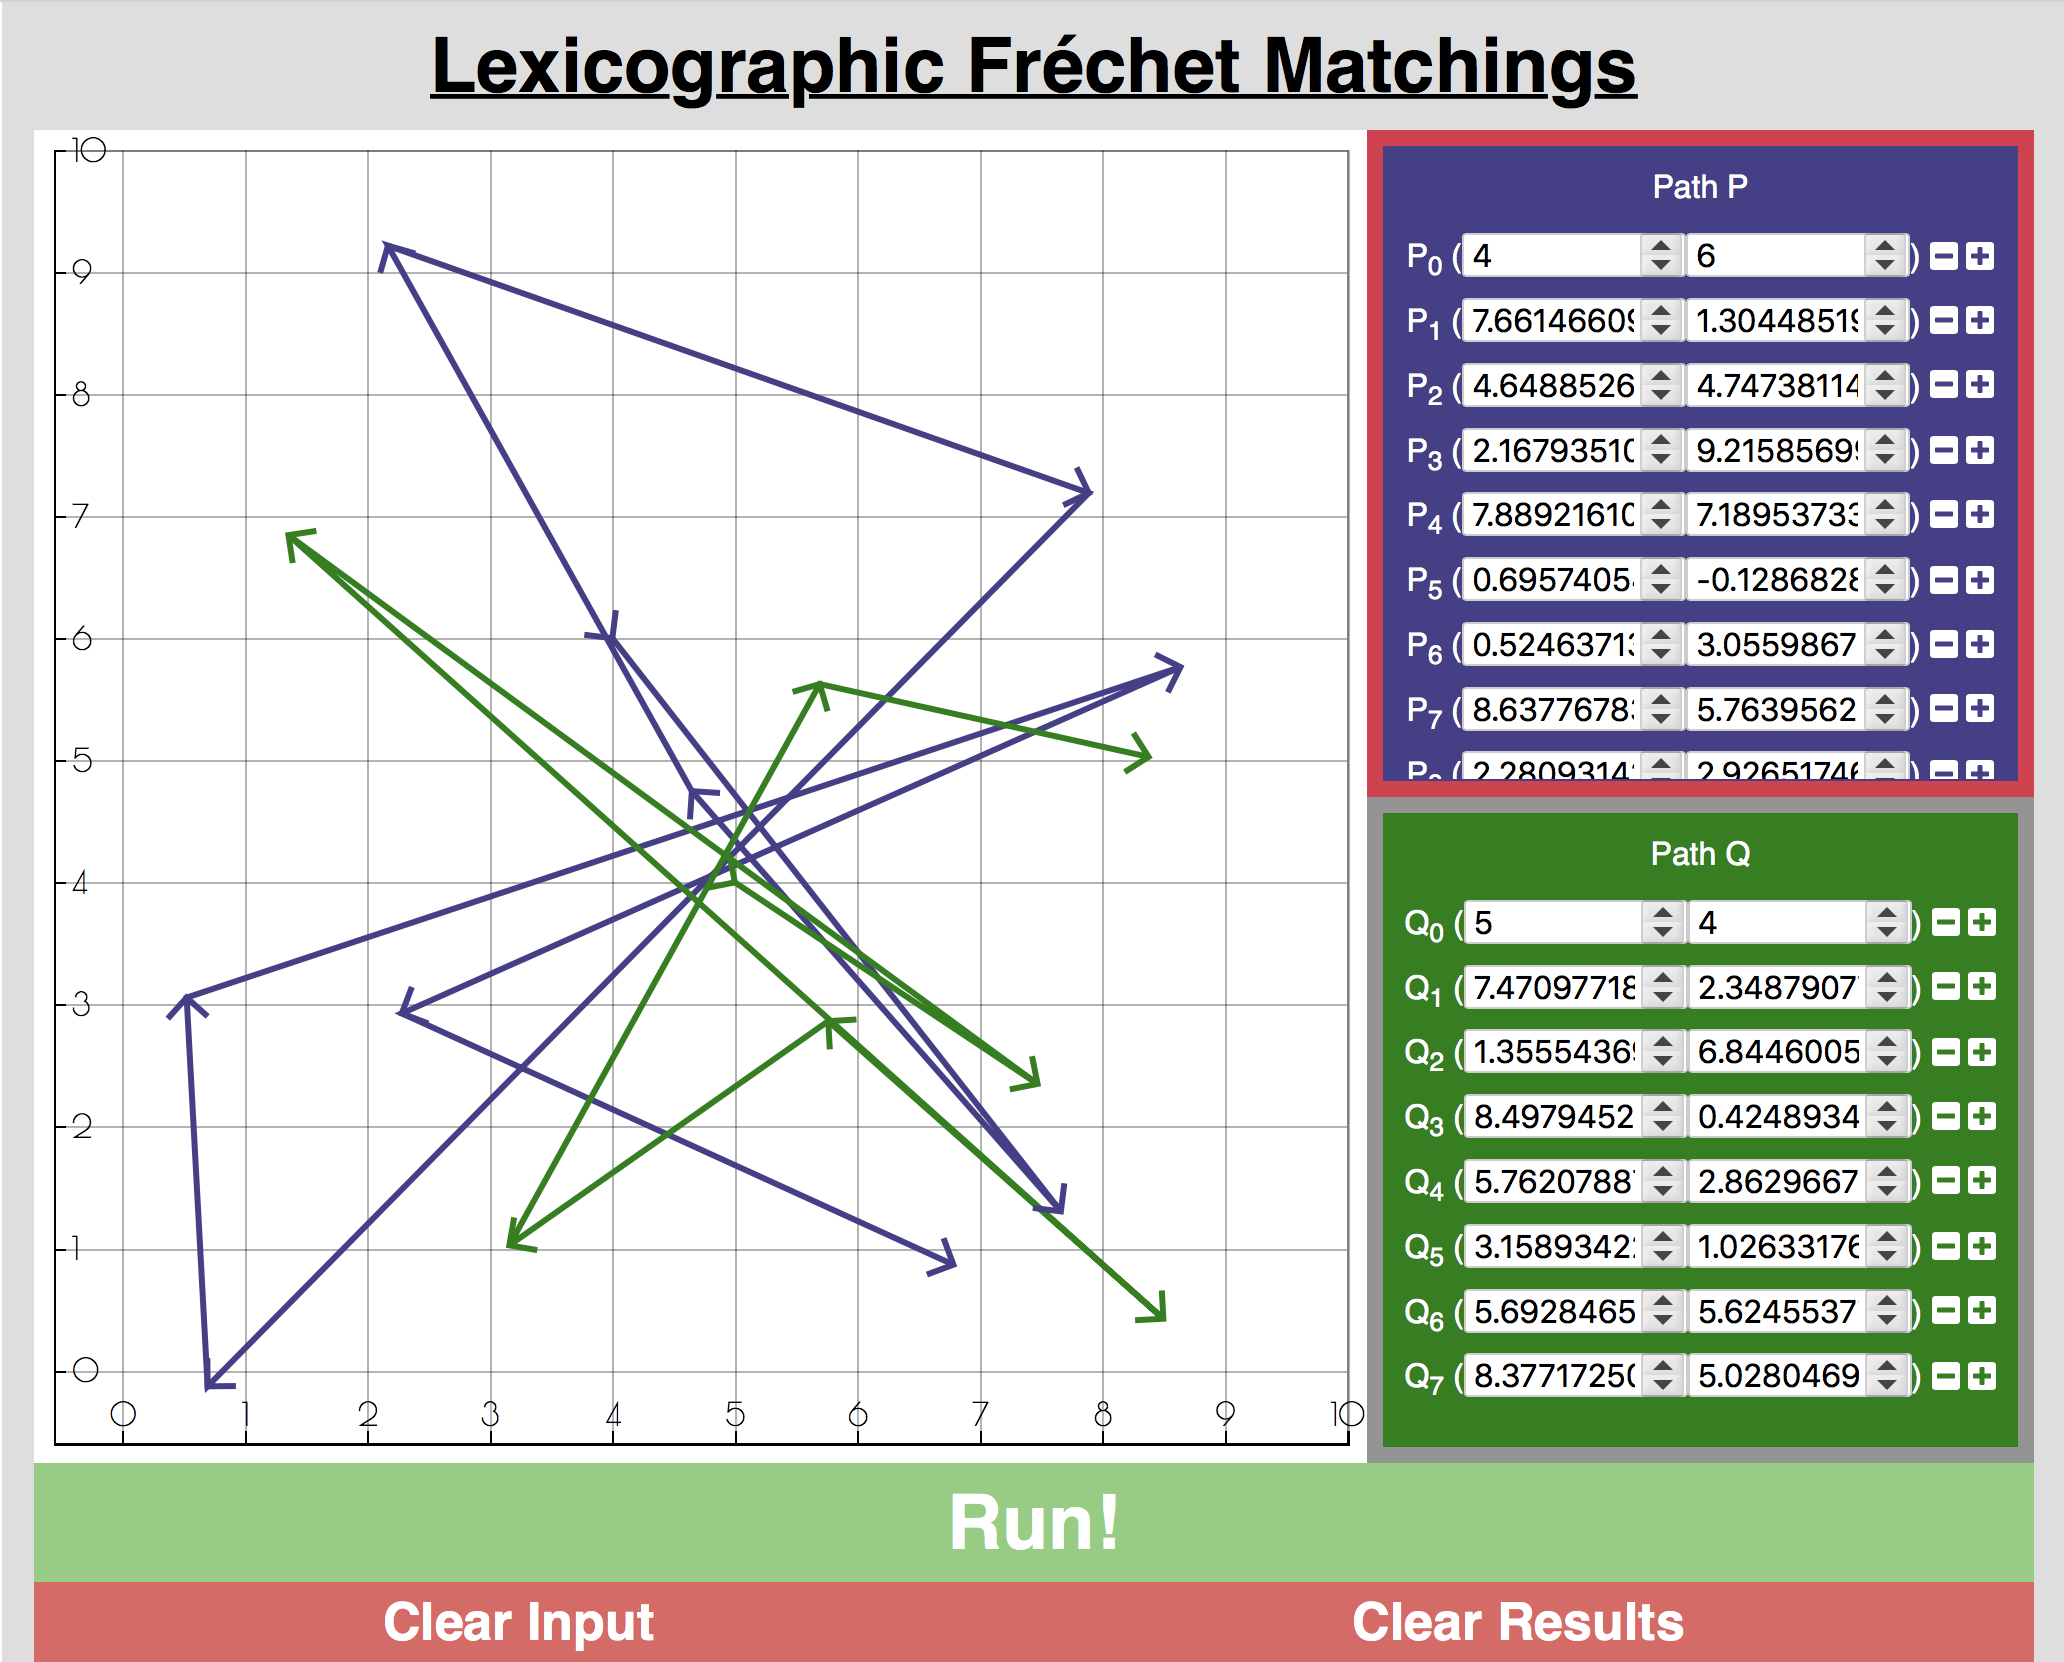
\includegraphics[width=0.8\textwidth]{webapp_input.png}
	\end{figure}
	
	\item Press ``Run". The frontend contacts the python backend where the algorithms are executed. When the computations finish, the results are returned to the frontend and displayed in three charts.

	\item If necessary select or deselect options like showing the free-space diagram, 
	
	\begin{figure}[H]
		\centering
		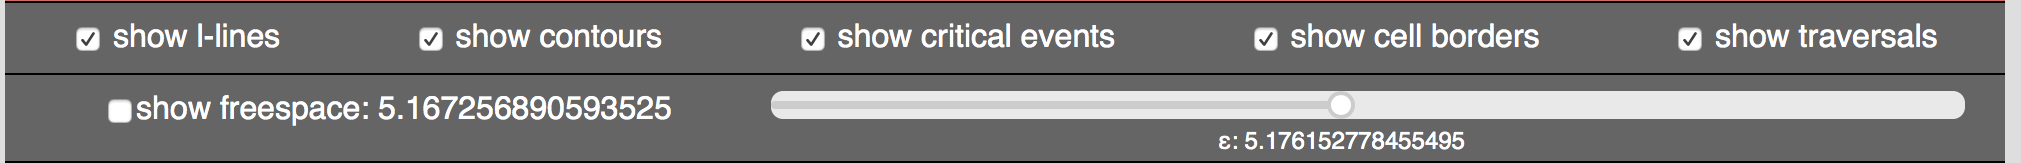
\includegraphics[width=1.0\textwidth]{webapp_options.png}
	\end{figure}
	
	\item View the height diagram $\delta$ as a contourmap with critical events and traversals overlaid.
	
	
	\begin{figure}[H]
		\centering
		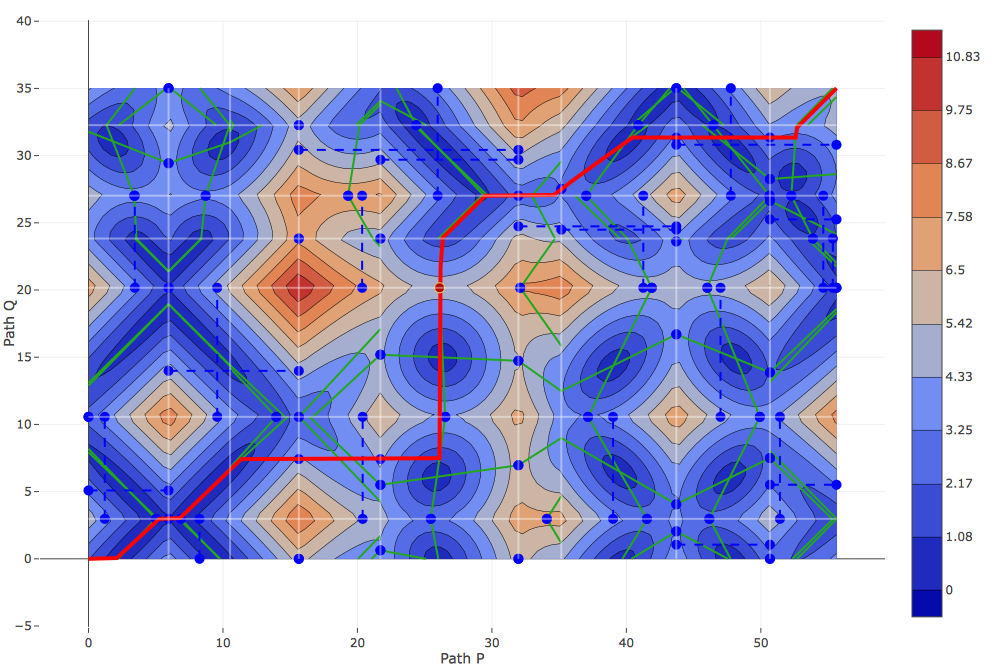
\includegraphics[width=0.7\textwidth]{webapp_2d.png}
	\end{figure}
	
	\item View the height diagram $\delta$ as a 3D model with critical events and traversals overlaid.
	
	\begin{figure}[H]
		\centering
		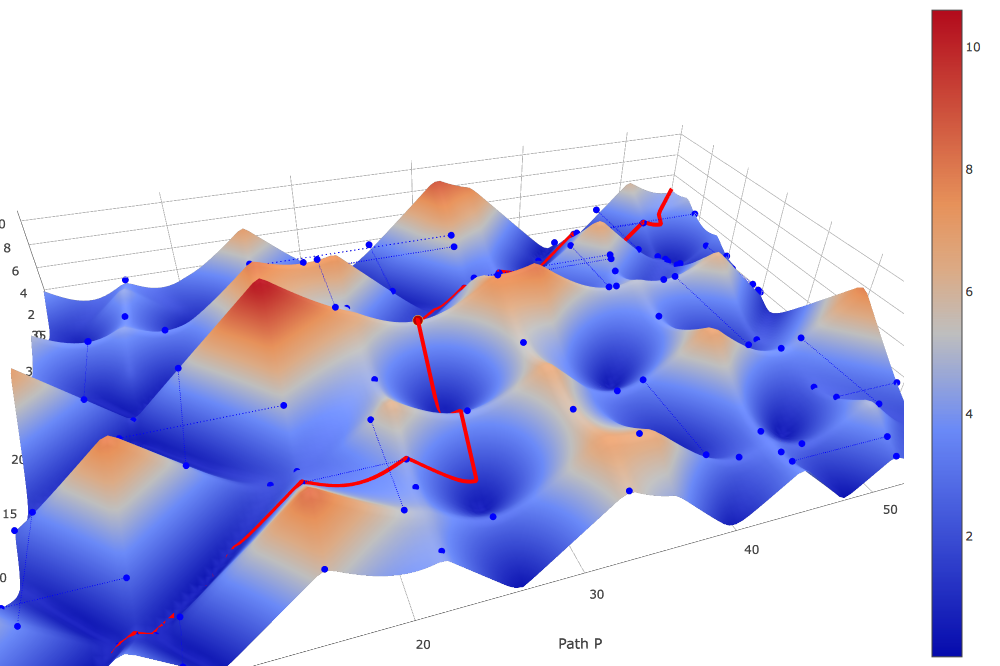
\includegraphics[width=0.7\textwidth]{webapp_3d.png}
	\end{figure}
	
	\item View the cross-sections and profiles of traversals.
	
	\begin{figure}[H]
		\centering
		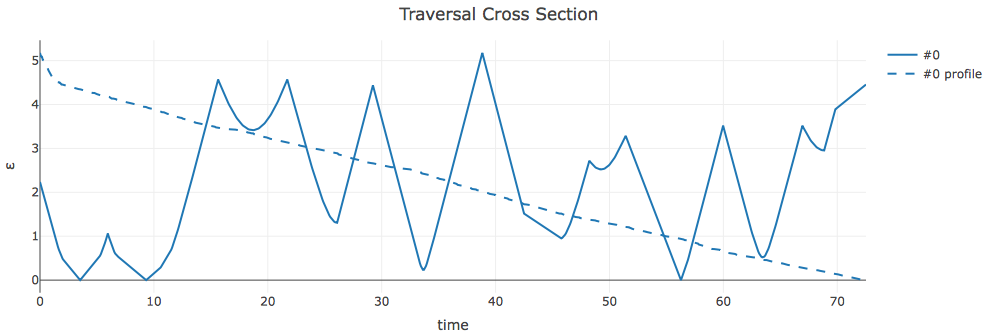
\includegraphics[width=0.7\textwidth]{webapp_cps.png}
	\end{figure}
	
	
	
\end{enumerate}


